\documentclass[11pt]{article}
\usepackage[margin=1in]{geometry}
\usepackage[T1]{fontenc}
\usepackage{lmodern,amsmath,amssymb,amsthm,booktabs,tikz}
\usepackage[title]{appendix}
\usepackage[colorlinks=true,linkcolor=blue,citecolor=blue,urlcolor=blue]{hyperref}
\hypersetup{pdfauthor={P. Graham},pdftitle={A subdivided 6-clique breaks a conjectured sum bound for independent monophonic-position colorings}}
\newtheorem{theorem}{Theorem}
\newtheorem{lemma}[theorem]{Lemma}
\theoremstyle{remark}
\newtheorem*{remark}{Remark}
\newcommand{\chimp}{\chi_{\mathrm{mp}_{\mathrm{i}}}}
\title{A subdivided 6-clique breaks a conjectured sum bound for
independent monophonic-position colorings}
\author{P. Graham\\ \small\url{https://orcid.org/0009-0007-8493-1505}}
\date{November 3, 2026}
\begin{document}
\maketitle
\begin{abstract}
A set of vertices of a graph is in monophonic position if no induced path
contains three of its vertices. Ullas Chandran S. V., Gabriele Di Stefano,
S. Haritha, Elias John Thomas and James Tuite introduced colorings whose
color classes are such sets, and the variant whose classes are also
independent. They showed that the monophonic-position chromatic numbers of
an $n$-vertex graph and of its complement sum to at most $n+1$, and
conjectured the same Nordhaus--Gaddum bound for the independent variant;
they report a computer search by Grahame Erskine confirming their
conjecture for all graphs with at most ten vertices. We show that the
independent monophonic sum bound fails. Subdividing every edge of the
complete graph $K_6$ once gives a graph $H$ on 21 vertices that needs at
least eight independent monophonic-position color classes, while its
complement needs at least fifteen, so the sum is at least 23. The proof
classifies the independent monophonic-position sets of $H$ and shows by
counting that seven color classes cannot cover $H$. The lower bounds are
also confirmed by SAT-solver proofs checked with a formally verified
checker.

This work has not yet been reviewed by experts.
The proofs, the code and the text were produced by AI models (from OpenAI
and Anthropic), working under the author's direction.
\end{abstract}
\medskip
\noindent\textbf{2020 Mathematics Subject Classification:} 05C15, 05C38.\\
\textbf{Keywords:} monophonic position, graph coloring, Nordhaus--Gaddum bound.

\section{Introduction}
All graphs are finite, simple and undirected. An induced path has distinct
vertices, with adjacency precisely between consecutive vertices. A
monophonic-position set meets every induced path in at most two vertices.
Following Chandran, Di Stefano, Haritha, Thomas and Tuite
\cite[Definition 2.3]{position}, write $\chimp(G)$ for the minimum number
of independent monophonic-position sets partitioning $V(G)$ (color
classes may be empty), the independent monophonic-position chromatic
number of $G$. Dropping independence gives the monophonic-position
chromatic number $\chi_{\mathrm{mp}}(G)$, and replacing induced paths by
shortest paths gives the general-position analogues. Both properties
pass to subsets: a subset of an independent monophonic-position set is
again one.

Chandran et al.\ proposed Nordhaus--Gaddum relations for these
colorings, after the classical bound $\chi(G)+\chi(\overline G)\leq n+1$
for the chromatic number \cite{nordhaus}. From their Lemma 4.1, the remark
before their Conjecture 9.3 derives, for every graph $G$ of order $n$,
\[
 \chi_{\mathrm{mp}}(G)+\chi_{\mathrm{mp}}(\overline G)\leq n+1,
\]
and the same for general position; it adds that ``up to order nine the
only example of equality is $C_5$ for $\chi_{\mathrm{mp}}$''.
Conjecture 9.3 asserts that for general position and for monophonic
position alike, the independent parameters satisfy the same sum bound
and a product bound. For monophonic position its sum part reads
\begin{equation}\label{eq:conjecture}
 \chimp(G)+\chimp(\overline G)\leq n+1.
\end{equation}
The paragraph after the conjecture states: ``It is true for all graphs
with up to ten vertices, as shown by a computer search by Erskine'',
citing a 2021 private communication from Grahame Erskine. The statements
cited here are numbered alike in arXiv version 2 and the published
version of \cite{position}.

Let $H$ be the graph obtained from $K_6$ by subdividing every edge once.
Its original vertices form $A=\{0,1,\ldots,5\}$ and its subdivision
vertices form $B=\{b_{ij}:0\leq i<j\leq5\}$, where we write
$b_{ji}=b_{ij}$; each $b_{ij}$ is adjacent exactly to $i$ and $j$. Thus
$H$ has 21 vertices and 30 edges (Figure~\ref{fig:H}). Both $H$ and
$\overline H$ are connected, so the convention of \cite{position} for
disconnected graphs plays no role.

\begin{theorem}\label{thm:main}
For the graph $H$ just defined,
\[
 \chimp(H)\geq8,\qquad \chimp(\overline H)\geq15.
\]
Consequently $\chimp(H)+\chimp(\overline H)\geq23>|V(H)|+1$, so $H$
violates \eqref{eq:conjecture}.
\end{theorem}

Theorem~\ref{thm:main} disproves the monophonic sum part
\eqref{eq:conjecture} of Conjecture 9.3; the general-position sum part
and both product parts remain open. Thus, for monophonic position, the
sum bound proved without independence does not extend to the
independent parameter. The counterexample needs only these lower
bounds; the remark in Section~\ref{sec:proof} gives colorings attaining
them. We do not know
whether a smaller counterexample exists. Monophonic position sets in
Cartesian and lexicographic products are studied in \cite{products}; we
do not use those results. Appendix~\ref{app:prior} lists further related
work.

\begin{figure}[ht]
\centering
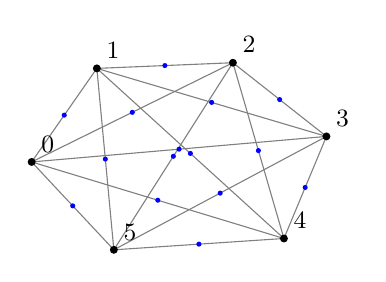
\begin{tikzpicture}[scale=.72]
\draw[gray] (0.65,-2.2) -- (1.225,-1.375);
\draw[gray] (0.65,-2.2) -- (2.425,-1.325);
\draw[gray] (0.65,-2.2) -- (3.25,-1.975);
\draw[gray] (0.65,-2.2) -- (2.875,-2.875);
\draw[gray] (0.65,-2.2) -- (1.375,-2.975);
\draw[gray] (1.8,-0.55) -- (1.225,-1.375);
\draw[gray] (1.8,-0.55) -- (3.0,-0.5);
\draw[gray] (1.8,-0.55) -- (3.825,-1.15);
\draw[gray] (1.8,-0.55) -- (3.45,-2.05);
\draw[gray] (1.8,-0.55) -- (1.95,-2.15);
\draw[gray] (4.2,-0.45) -- (2.425,-1.325);
\draw[gray] (4.2,-0.45) -- (3.0,-0.5);
\draw[gray] (4.2,-0.45) -- (5.025,-1.1);
\draw[gray] (4.2,-0.45) -- (4.65,-2.0);
\draw[gray] (4.2,-0.45) -- (3.15,-2.1);
\draw[gray] (5.85,-1.75) -- (3.25,-1.975);
\draw[gray] (5.85,-1.75) -- (3.825,-1.15);
\draw[gray] (5.85,-1.75) -- (5.025,-1.1);
\draw[gray] (5.85,-1.75) -- (5.475,-2.65);
\draw[gray] (5.85,-1.75) -- (3.975,-2.75);
\draw[gray] (5.1,-3.55) -- (2.875,-2.875);
\draw[gray] (5.1,-3.55) -- (3.45,-2.05);
\draw[gray] (5.1,-3.55) -- (4.65,-2.0);
\draw[gray] (5.1,-3.55) -- (5.475,-2.65);
\draw[gray] (5.1,-3.55) -- (3.6,-3.65);
\draw[gray] (2.1,-3.75) -- (1.375,-2.975);
\draw[gray] (2.1,-3.75) -- (1.95,-2.15);
\draw[gray] (2.1,-3.75) -- (3.15,-2.1);
\draw[gray] (2.1,-3.75) -- (3.975,-2.75);
\draw[gray] (2.1,-3.75) -- (3.6,-3.65);
\fill[black] (0.65,-2.2) circle (0.07);
\node[above right] at (0.65,-2.2) {\small 0};
\fill[black] (1.8,-0.55) circle (0.07);
\node[above right] at (1.8,-0.55) {\small 1};
\fill[black] (4.2,-0.45) circle (0.07);
\node[above right] at (4.2,-0.45) {\small 2};
\fill[black] (5.85,-1.75) circle (0.07);
\node[above right] at (5.85,-1.75) {\small 3};
\fill[black] (5.1,-3.55) circle (0.07);
\node[above right] at (5.1,-3.55) {\small 4};
\fill[black] (2.1,-3.75) circle (0.07);
\node[above right] at (2.1,-3.75) {\small 5};
\fill[blue] (1.225,-1.375) circle (0.045);
\fill[blue] (2.425,-1.325) circle (0.045);
\fill[blue] (3.25,-1.975) circle (0.045);
\fill[blue] (2.875,-2.875) circle (0.045);
\fill[blue] (1.375,-2.975) circle (0.045);
\fill[blue] (3.0,-0.5) circle (0.045);
\fill[blue] (3.825,-1.15) circle (0.045);
\fill[blue] (3.45,-2.05) circle (0.045);
\fill[blue] (1.95,-2.15) circle (0.045);
\fill[blue] (5.025,-1.1) circle (0.045);
\fill[blue] (4.65,-2.0) circle (0.045);
\fill[blue] (3.15,-2.1) circle (0.045);
\fill[blue] (5.475,-2.65) circle (0.045);
\fill[blue] (3.975,-2.75) circle (0.045);
\fill[blue] (3.6,-3.65) circle (0.045);
\end{tikzpicture}
\caption{The graph $H$. Original vertices are black; subdivision vertices
are blue, each joined to the two original vertices of the edge of $K_6$ it
subdivides. Crossings without a dot are not vertices.}\label{fig:H}
\end{figure}

\section{Proof of Theorem~\ref{thm:main}}\label{sec:proof}
The main step is a classification: every independent
monophonic-position set of $H$ with at least three vertices lies among
the five subdivision vertices adjacent to a single original vertex. The
lower bound for $H$ then follows by counting how many original and
subdivision vertices a collection of such sets can cover. The lower bound
for $\overline H$ is immediate, because $B$ is a clique there.

For $i\in A$, let $C_i=N_H(i)=\{b_{ij}:j\in A\setminus\{i\}\}$ be the
star set at $i$, the five subdivision vertices adjacent to $i$. We call
$\mathcal C$ the catalog: it consists of the six star sets and all
independent pairs of $H$ not contained in a star set. There are 120 such
pairs: $H$ has $\binom{21}{2}-30=180$ independent pairs, and the star sets
contain $6\binom{5}{2}=60$ distinct pairs.

\begin{lemma}[Classification of color classes]\label{lem:catalog}
Each member of $\mathcal C$ is an independent monophonic-position set of
$H$. Every independent monophonic-position set of $H$ is contained in a
member of $\mathcal C$.
\end{lemma}
\begin{proof}
A set of at most two vertices meets every path in at most two vertices,
so every independent pair of $H$ is an independent monophonic-position
set. Each $C_i$ is independent. If an induced path omits $i$, any vertex
of $C_i$ on it must be an endpoint, since an interior $b_{ij}$ needs both
neighbors $i,j$. If the path contains $i$, all its vertices from $C_i$
must be consecutive to $i$, to avoid chords. In either case it contains
at most two vertices of $C_i$.

We show that every independent triple not contained in a star set lies
on an induced path. A simple path in $K_6$, with its edges subdivided,
is induced in $H$. One may also append a subdivision vertex at either
end when its other neighbor is absent from the path. Up to renaming, an
independent triple that meets $A$ has one of the four forms below, in
which distinct letters denote distinct original vertices: independence
forces each subdivision vertex of the triple to avoid the triple's
original vertices, and two subdivision vertices share one original
vertex or none. Each row gives an induced path containing the triple:
\[
\begin{array}{c|l}
\text{Triple} & \text{Induced path} \\\hline
\{a,a',c\} & a,b_{ac},c,b_{ca'},a' \\
\{a,a',b_{cd}\} & a,b_{ac},c,b_{cd},d,b_{da'},a' \\
\{a,b_{cd},b_{df}\} & a,b_{ac},c,b_{cd},d,b_{df},f \\
\{a,b_{cd},b_{ef}\} & a,b_{ac},c,b_{cd},d,b_{de},e,b_{ef}
\end{array}
\]
A triple in $B$ corresponds to three edges of $K_6$. Unless they share
a common endpoint, their graph is a triangle, a three-edge path, a
two-edge path and a disjoint edge, or three disjoint edges. The required
paths, in the same order, are
\[
\begin{array}{c|l}
\text{Edges of }K_6 & \text{Induced path in }H \\\hline
xy,xz,yz & b_{xy},x,b_{xz},z,b_{yz} \\
xy,yz,zt & x,b_{xy},y,b_{yz},z,b_{zt},t \\
xy,yz,uv & x,b_{xy},y,b_{yz},z,b_{zu},u,b_{uv},v \\
xy,zu,vw & x,b_{xy},y,b_{yz},z,b_{zu},u,b_{uv},v,b_{vw},w
\end{array}
\]
Thus every triple in an independent monophonic-position set $S$ lies
in a star set. If $|S|\geq3$, fix two elements of one such triple and
its star set $C_i$. For each remaining element of $S$, the triple formed
with that pair lies in a star set. Since $|C_i\cap C_j|=1$ for $i\ne j$,
that star set must again be $C_i$. Hence $S\subseteq C_i$. Sets of size
at most two are contained in members of $\mathcal C$ as well.
\end{proof}

\begin{proof}[Proof of Theorem~\ref{thm:main}]
By Lemma~\ref{lem:catalog}, extending every color class of a coloring of
$H$ to a member of $\mathcal C$ containing it gives a cover of $V(H)$ by
no more members of $\mathcal C$ than colors. Remove repeated members.
Suppose the cover uses $c$ star sets and $p_{AA}$, $p_{AB}$, $p_{BB}$
pairs with, respectively, both vertices in $A$, one vertex in each of
$A$ and $B$, and both vertices in $B$; put $p=p_{AA}+p_{AB}+p_{BB}$. The
star sets lie in $B$, so only pairs cover $A$: $2p_{AA}+p_{AB}\geq6$. The
subdivision vertices whose two original endpoints are outside the $c$
star centers number $\binom{6-c}{2}$. They too must be covered by pairs,
giving $p_{AB}+2p_{BB}\geq\binom{6-c}{2}$. Adding yields
\[
 c+p\ \geq\ c+3+\frac12\binom{6-c}{2}
 =\frac{15}{2}+\frac{(c-3)(c-4)}4\ \geq\ \frac{15}{2},
\]
since $c$ is an integer between zero and six. The number of classes is
an integer, so $\chimp(H)\geq8$.

In $\overline H$, the fifteen vertices of $B$ form a clique, so an
independent set of $\overline H$ contains at most one of them. Hence
$\chimp(\overline H)\geq15$.
\end{proof}

\begin{remark}
Both bounds are attained. Partition $B$ into the five nonempty sets
$D_i=C_i\setminus\bigcup_{j<i}C_j$ for $0\leq i\leq4$, and partition $A$
into $\{0,1\},\{2,3\},\{4,5\}$. Each $D_i$ is a subset of a star set, so
by Lemma~\ref{lem:catalog} and heredity these eight classes are
independent monophonic-position sets. Every $b_{ij}$ with $i<j$ belongs
to $D_i$, so they cover all vertices, and $\chimp(H)=8$. In $\overline
H$, take the six classes
\[
 \{0,b_{01}\},\ \{1,b_{12}\},\ \{2,b_{23}\},\
 \{3,b_{34}\},\ \{4,b_{45}\},\ \{5,b_{05}\},
\]
and the nine remaining vertices of $B$ as singletons. Each pair is an
edge of $H$, hence independent in $\overline H$, and any set of size at
most two is a monophonic-position set. These fifteen classes give
$\chimp(\overline H)=15$.
\end{remark}

\section{Verification and reproducibility}
The proof above is complete by hand. As an independent check, the
completeness of $\mathcal C$ and the absence of a cover of $H$ by seven
members of $\mathcal C$ are encoded as Boolean satisfiability problems,
the cardinality bound by Sinz's sequential counter~\cite{sinz}; the
same is done for $\overline H$, with its catalog of the 30 edges of $H$
and covers by fourteen members. The SAT solver CaDiCaL~\cite{cadical}
produced proofs of unsatisfiability. Wetzler, Heule and Hunt's
drat-trim~\cite{drat} checks them and converts them to LRAT proofs,
which Tan, Heule and Myreen's cake\_lpr~\cite{cake}, a checker verified
in the CakeML system, checks independently. The verified checker checks
propositional proofs, not their graph-theoretic interpretation; that
step relies on the Python code that builds the formulas from $H$. The
code, the exact encodings, the certificates and the instructions are in
the folder \texttt{checks/} of the result's repository.

\begin{appendices}
\section{Related work}\label{app:prior}
The prior-work search was bounded, and this list is selected; the
checking notes in the result's repository (\texttt{checks/README.md})
record the versions read and not read and why each source is excluded.
In the versions read, none of the following works treats the sum
\eqref{eq:conjecture}.

\begin{enumerate}\setlength{\itemsep}{2pt}
\item Thomas, Chandran, Tuite and Di Stefano~\cite{monophonic}: Section 5
defines the ``independent monophonic position'' number, the largest size
of one such set.
\item Thomas and Chandran~\cite{independent}: ``An independent set $S$ of
vertices in a graph $G$ is an independent position set if no three
vertices of $S$ lie on a common geodesic.''
\item Sadiquali and Sudhahar~\cite{sadiquali}, a different parameter
under a similar name: ``the minimum size of an independent monophonic
set''.
\item Chandran, Klav\v{z}ar, Neethu and Tuite~\cite{products}: ``the
monophonic position number is studied on Cartesian and lexicographic
products of graphs''.
\item Tuite, Thomas and Chandran~\cite{extremal}: ``we investigate some
extremal problems for these parameters''.
\item Di Stefano, Klav\v{z}ar, Krishnakumar, Tuite and
Yero~\cite{lower}: the ``smallest maximal general position set''.
\item Klav\v{z}ar, Tian and Tuite~\cite{builder}: ``a general position
set is built through adversarial play''.
\item Thomas, Chandran, Tuite and Di Stefano~\cite{mycielski}: ``we
investigate the general position numbers of the Mycielskian of
graphs''.
\item Ir\v{s}i\v{c}, Klav\v{z}ar, Rus and Tuite~\cite{polynomials}:
coefficients giving ``the number of distinct general position sets of
$G$ with cardinality'' $i$.
\item Kruft Welton, Khudairi and Tuite~\cite{lowerproducts}: ``the lower
general position problem asks for a smallest maximal general position
set''.
\item Araujo, Dourado, Protti and Sampaio~\cite{convexities}, on the
iteration time and the general position number in graph convexities.
\item Hamed-Labbafian, Henning and Tavakoli~\cite{edge}, on edge general
position.
\item Yan~\cite{yan}: ``No circulant graph of order 15 has both diameter
2 and monophonic position number 2''.
\end{enumerate}
\end{appendices}

\begin{thebibliography}{99}
\bibitem{position}
Ullas Chandran S. V., Gabriele Di Stefano, S. Haritha, Elias John Thomas
and James Tuite, \emph{Colouring a graph with position sets},
Ars Mathematica Contemporanea 26 (2026), \#P4.06.
\href{https://doi.org/10.26493/1855-3974.3454.a3c}{doi:10.26493/1855-3974.3454.a3c}.
\href{https://arxiv.org/abs/2408.13494v2}{arXiv:2408.13494v2}.

\bibitem{nordhaus}
E. A. Nordhaus and J. W. Gaddum, \emph{On complementary graphs},
American Mathematical Monthly 63 (1956), 175--177.
\href{https://doi.org/10.2307/2306658}{doi:10.2307/2306658}.

\bibitem{products}
Ullas Chandran S. V., Sandi Klav\v{z}ar, P. K. Neethu and James Tuite,
\emph{Monophonic position sets of Cartesian and lexicographic products
of graphs}, Computational and Applied Mathematics 46 (2027), article 44;
published online September 11, 2026.
\href{https://doi.org/10.1007/s40314-026-03901-3}{doi:10.1007/s40314-026-03901-3}.
\href{https://arxiv.org/abs/2412.09837v3}{arXiv:2412.09837v3}.

\bibitem{monophonic}
Elias John Thomas, Ullas Chandran S. V., James Tuite and Gabriele Di
Stefano, \emph{On monophonic position sets in graphs}, Discrete Applied
Mathematics 354 (2024), 72--82.
\href{https://doi.org/10.1016/j.dam.2023.02.021}{doi:10.1016/j.dam.2023.02.021}.
\href{https://arxiv.org/abs/2012.10330v4}{arXiv:2012.10330v4}.

\bibitem{independent}
Elias John Thomas and Ullas Chandran S. V., \emph{On independent position
sets in graphs}, Proyecciones 40(2) (2021), 385--398.
\href{https://doi.org/10.22199/issn.0717-6279-2021-02-0023}{doi:10.22199/issn.0717-6279-2021-02-0023}.

\bibitem{sadiquali}
A. Sadiquali and P. Arul Paul Sudhahar, \emph{Independent Monophonic Sets
in Graphs}, Mapana Journal of Sciences 18(3) (2019), 33--44.
\href{https://doi.org/10.12723/mjs.50.3}{doi:10.12723/mjs.50.3}.

\bibitem{extremal}
James Tuite, Elias John Thomas and Ullas Chandran S. V.,
\emph{On some extremal position problems for graphs}, Ars Mathematica
Contemporanea 25 (2025), \#P1.09.
\href{https://doi.org/10.26493/1855-3974.3094.bc6}{doi:10.26493/1855-3974.3094.bc6}.
\href{https://arxiv.org/abs/2106.06827}{arXiv:2106.06827}.

\bibitem{lower}
Gabriele Di Stefano, Sandi Klav\v{z}ar, Aditi Krishnakumar, James Tuite
and Ismael G. Yero, \emph{Lower general position sets in graphs},
Discussiones Mathematicae Graph Theory 45(2) (2025), from page 509.
\href{https://doi.org/10.7151/dmgt.2542}{doi:10.7151/dmgt.2542}.

\bibitem{builder}
Sandi Klav\v{z}ar, Jing Tian and James Tuite, \emph{Builder-Blocker
general position games}, Communications in Combinatorics and Optimization
11(2) (2026), 465--486.\newline
\href{https://doi.org/10.22049/cco.2024.29122.1854}{doi:10.22049/cco.2024.29122.1854}.
\href{https://arxiv.org/abs/2310.19949v2}{arXiv:2310.19949v2}.

\bibitem{mycielski}
Elias John Thomas, Ullas Chandran S. V., James Tuite and Gabriele Di
Stefano, \emph{On the general position number of Mycielskian graphs},
Discrete Applied Mathematics 353 (2024), 29--43.
\href{https://doi.org/10.1016/j.dam.2024.03.015}{doi:10.1016/j.dam.2024.03.015}.
\href{https://arxiv.org/abs/2203.08170v2}{arXiv:2203.08170v2}.

\bibitem{polynomials}
Vesna Ir\v{s}i\v{c}, Sandi Klav\v{z}ar, Gregor Rus and James Tuite,
\emph{General position polynomials}, Results in Mathematics 79 (2024),
article 110.
\href{https://doi.org/10.1007/s00025-024-02133-3}{doi:10.1007/s00025-024-02133-3}.

\bibitem{lowerproducts}
Eartha Kruft Welton, Sharif Khudairi and James Tuite, \emph{Lower general
position in Cartesian products}, Communications in Combinatorics and
Optimization 10(1) (2025), 111--126.
\href{https://doi.org/10.22049/cco.2024.29171.1879}{doi:10.22049/cco.2024.29171.1879}.
\href{https://arxiv.org/abs/2404.19451v1}{arXiv:2404.19451v1}.

\bibitem{convexities}
Julio Araujo, Mitre C. Dourado, F\'abio Protti and Rudini Sampaio,
\emph{The iteration time and the general position number in graph
convexities}, Applied Mathematics and Computation 487 (2025), 129084.
\href{https://doi.org/10.1016/j.amc.2024.129084}{doi:10.1016/j.amc.2024.129084}.
\href{https://arxiv.org/abs/2305.00467v5}{arXiv:2305.00467v5}.

\bibitem{edge}
Zahra Hamed-Labbafian, Michael A. Henning and Mostafa Tavakoli,
\emph{Edge general position in graphs: Graph products, integer linear
programming and some applications}, Discrete Applied Mathematics 386
(2026), 1--8.
\href{https://doi.org/10.1016/j.dam.2026.01.008}{doi:10.1016/j.dam.2026.01.008}.

\bibitem{yan}
Zeyu Yan, \emph{Monophonic Position in Circulant Graphs: A
Counterexample, an Induced-Path Criterion, and an Infinite Family},
August 18, 2026.
\href{https://doi.org/10.5281/zenodo.21995203}{doi:10.5281/zenodo.21995203}.

\bibitem{cadical}
Armin Biere, Tobias Faller, Katalin Fazekas, Mathias Fleury,
Nils Froleyks and Florian Pollitt, \emph{CaDiCaL 2.0}, CAV 2024,
Lecture Notes in Computer Science 14681, 133--152.
\href{https://cca.informatik.uni-freiburg.de/papers/BiereFallerFazekasFleuryFroleyksPollitt-CAV24.pdf}{Author manuscript}.

\bibitem{drat}
Nathan Wetzler, Marijn J. H. Heule and Warren A. Hunt, Jr.,
\emph{DRAT-trim: Efficient Checking and Trimming Using Expressive
Clausal Proofs}, SAT 2014, Lecture Notes in Computer Science 8561,
422--429.
\href{https://www.cs.cmu.edu/~mheule/publications/drat-trim.pdf}{Author manuscript}.

\bibitem{cake}
Yong Kiam Tan, Marijn J. H. Heule and Magnus O. Myreen,
\emph{cake\_lpr: Verified Propagation Redundancy Checking in CakeML},
TACAS 2021, Lecture Notes in Computer Science 12652, 223--241.
\href{https://doi.org/10.1007/978-3-030-72013-1_12}{doi:10.1007/978-3-030-72013-1\_12}.

\bibitem{sinz}
Carsten Sinz, \emph{Towards an Optimal CNF Encoding of Boolean
Cardinality Constraints}, CP 2005, Lecture Notes in Computer Science
3709, 827--831.
\href{https://doi.org/10.1007/11564751_73}{doi:10.1007/11564751\_73}.
\end{thebibliography}

\end{document}
